\subsubsection{UC13 - Salvataggio di un nuovo dizionario dati nel sistema}\label{UC13}

\begin{figure}[H]
  \centering
  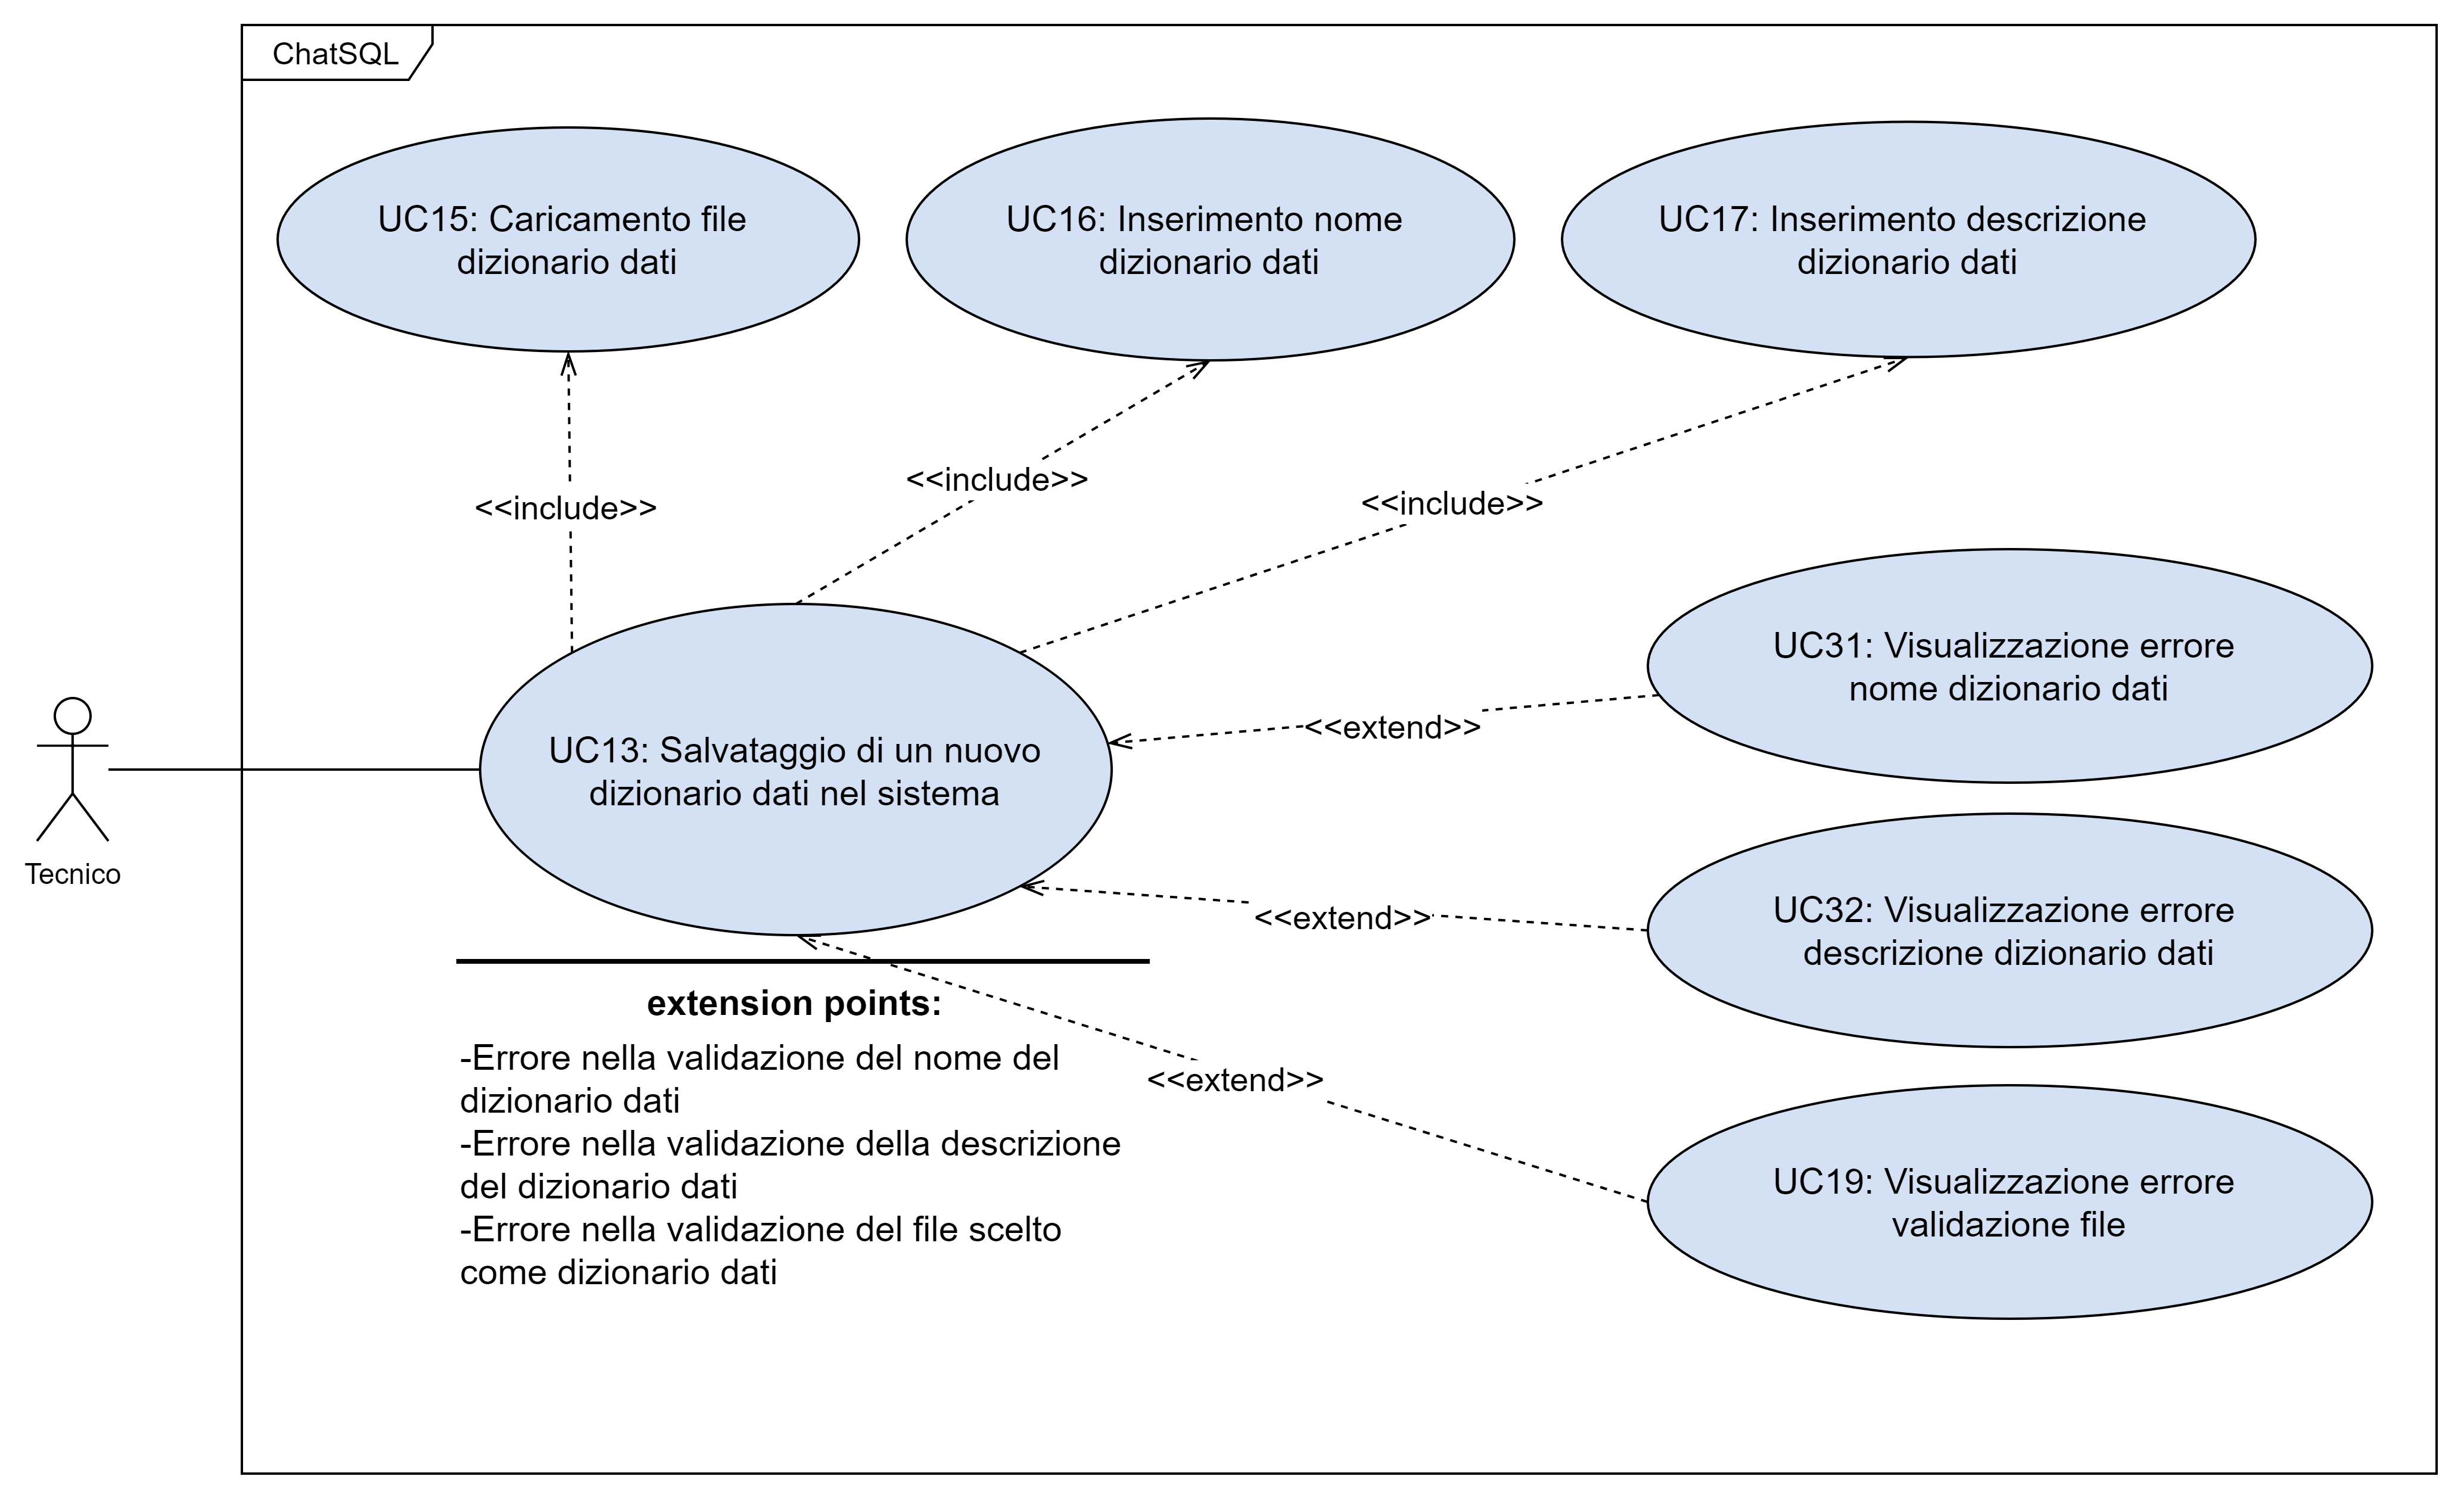
\includegraphics[width=0.90\textwidth]{assets/uc13.png}
  \caption{UC13}
\end{figure}

\paragraph*{Descrizione}
Il salvataggio di un \glossario{dizionario dati} corrisponde alla procedura di inserimento di un dizionario e delle sue informazioni all'interno del sistema.

\paragraph*{Attori principali}
Tecnico

\paragraph*{Precondizioni}
\begin{itemize}
  \item Il sistema è attivo e funzionante;
  \item Il Tecnico ha effettuato l'autenticazione (\hyperref[UC1]{UC1});
\end{itemize}

\paragraph*{Postcondizioni}
\begin{itemize}
  \item Il \glossario{dizionario dati} è stato salvato con successo.
\end{itemize}

\paragraph*{Trigger}
Il Tecnico vuole aggiungere un nuovo \glossario{dizionario dati} nell'applicazione.

\paragraph*{Scenario principale}
\begin{enumerate}
  \item Il Tecnico inserisce il file, il nome e la descrizione del \glossario{dizionario dati};
  \item Il Tecnico richiede il salvataggio del \glossario{dizionario dati};
  \item Il \glossario{dizionario dati} viene salvato nel sistema;
  \item Il \glossario{dizionario dati} è disponibile a tutti gli utenti;
  \item Il \glossario{dizionario dati} può essere utilizzato per la generazione di \glossario{prompt}.
\end{enumerate}

\paragraph*{Scenario alternativo}
\begin{enumerate}
  \item Il sistema riscontra un errore durante la validazione del \glossario{dizionario dati};
  \item Viene visualizzato un messaggio d'errore esplicativo.
\end{enumerate}

\paragraph*{Inclusioni}
\begin{itemize}
  \item Caricamento file dizionario dati (\hyperref[UC15]{UC15});
  \item Inserimento nome dizionario dati (\hyperref[UC16]{UC16});
  \item Inserimento descrizione dizionario dati (\hyperref[UC17]{UC17}).
\end{itemize}

\paragraph*{Estensioni}
\begin{itemize}
  \item Visualizzazione errore validazione file (\hyperref[UC19]{UC19}).
  \begin{itemize}
    \item Extension point: errore nella validazione del file scelto come \glossario{dizionario dati};
    \item Condition: formato del file non valido, file troppo pesante, file non conforme allo schema predefinito.
  \end{itemize}
  \item Visualizzazione errore nome \glossario{dizionario dati} (\hyperref[UC31]{UC31}).
  \begin{itemize}
    \item Extension point: errore nella validazione del nome del \glossario{dizionario dati};
    \item Condition: formato del nome non corretto, nome già esistente.
  \end{itemize}
  \item Visualizzazione errore descrizione \glossario{dizionario dati} (\hyperref[UC32]{UC32}).
  \begin{itemize}
    \item Extension point: errore nella validazione della descrizione del \glossario{dizionario dati}.
  \end{itemize}
\end{itemize}
